\documentclass{article}

\usepackage{amsmath}
\usepackage{gensymb}
\usepackage{graphicx}
\usepackage[english]{babel}
\usepackage{framed}
\usepackage{array}
\usepackage{listings}
\usepackage{xcolor}
\usepackage[colorlinks = true,
            linkcolor = blue,
            urlcolor  = blue,
            citecolor = blue,
            anchorcolor = blue]{hyperref}
\usepackage{subfigure}
\usepackage{underscore}
\usepackage{caption}
\usepackage{fancyhdr} 
\usepackage{lastpage}  
\usepackage{geometry}
\usepackage{setspace} 
\usepackage{caption}    
\usepackage{mathtools}
\usepackage{tensor}     
\usepackage{adjustbox}
\usepackage{hhline}      
\onehalfspacing

\usepackage{color, colortbl}
\definecolor{LightCyan}{rgb}{0.88,1,1}

\geometry{top=1.5in}
\geometry{bottom=1.5in}
\geometry{left=1in}
\geometry{right=1in}

\renewcommand\contentsname{}
\renewcommand\listfigurename{}
\renewcommand\listtablename{}

\geometry{headheight=4cm}
\geometry{footskip=3cm}

\pagestyle{fancy}       
\fancyheadoffset{1in}
\fancyfootoffset{1in}  

\newcommand{\horrule}[1]{\rule{\linewidth}{#1}}
\newcommand{\MYhref}[3][blue]{\href{#2}{\color{#1}{#3}}}%

\graphicspath{ {Images/} }

\lhead{
\includegraphics[width=2cm]{reconso_patch}}
\chead{\LARGE{\textbf{Concept of Operations}}\vspace{0.5cm}}
\rhead{
\includegraphics[width=2cm]{usaf_patch}}

\lfoot{\vspace{-1.0cm} February 14, 2017}
\cfoot{
\includegraphics[height=2cm]{georgia_tech_logo}}
\rfoot{\vspace{-1.0cm} Page \thepage\ of \pageref{LastPage}}

\renewcommand{\headrulewidth}{2pt}
\renewcommand{\footrulewidth}{2pt}

\title{\vspace{2in} \textbf{Concept of Operations}}
\author{Team RECONSO}
\date{February 14, 2017}


\author{Presented to Air Force Research Lab, University Nanosat Program}

\begin{document}

\maketitle\thispagestyle{fancy}

\newpage

\section*{\center Approval}
\vspace{1in}
\begin{center}
	\begin{tabular}{p{3in}p{1in}}
		& \\ \hline
		Lyndy Axon & \hfill Date \\
		Chief Systems Engineer, Team RECONSO \\
		Georgia Institute of Technology \\
	\end{tabular}
\end{center}
\begin{center}
\begin{tabular}{p{3in}p{1in}}
    & \\ \hline
    Francis Park & \hfill Date \\
    Program Manager, Team RECONSO & \\
    Georgia Institute of Technology & \\
\end{tabular}
\end{center}
\vspace{0.5in}

\vspace{0.5in}
\begin{center}
\begin{tabular}{p{3in}p{1in}}
    & \\ \hline
    Dr. Marcus Holzinger & \hfill Date \\
    Principal Investigator, Team RECONSO \\
    Georgia Institute of Technology \\
\end{tabular}
\end{center}

\newpage


\section*{\centering Revisions}

\vspace{0.5in}
\begin{center}
\begin{tabular}{|c|c|c|c|}
    \hline
              &                   &              &            \\
    Revision  &  Description      &  Date        &  Approval  \\
              &                   &              &            \\ \hline
              &                   &              &            \\
    1.0       &  Initial Release  &  10/30/2014    &  10/30/2014  \\
              &                   	&              &            \\ \hline
              &       Add software            &              &            \\
    1.1       &     states to each   &  10/31/2014   &  10/31/2014 \\
              &        software mode           &              &            \\ \hline
              &                   &              &            \\
    1.2       &  Updated modes        &  11/23/2014  &  11/23/2014       \\
              &                   &              &            \\ \hline
              &       Updated            &              &            \\
    1.3       &       FSW flow         &  4/8/2015    &  4/8/2015       \\
              &        chart           &              &            \\ \hline
              &      Incorporating          &              &            \\
    2.0       &     AFRL edits           &  2/8/2016    &  2/10/2016       \\
              &     from Pre-PIR            &              &            \\ \hline
              &     Updated flow chart;          &              &            \\
	3.0       &     incorporated AFRL       &  2/14/2017    &  2/15/2017       \\
              &     edits from PIR         &              &            \\ \hline
\end{tabular}
\end{center}

\vspace{2cm}

\section*{\centering Team Contact}

\vspace{0.5in}
\begin{center}
\begin{tabular}{|c|c|c|}
    \hline
    Team Member       &  Role            &  Contact                 \\ \hhline{|=|=|=|}
    Lyndy Axon  &  Chief Systems Engineer     &  lyndyaxon@gatech.edu    \\ \hline
    Francis Park    & Program Mangaer  &  francis.park@gatech.edu  \\ \hline
    Eric Stoker-Spirt & ADCS Lead & stokerspirt@gatech.edu \\ \hline
    Jon Dolan	 & AVI Lead & jondolan@gatech.edu \\ \hline
    Baijun Desai & COM Lead & aakins6@gatech.edu \\ \hline
	Norris Nicholson & EGSE Lead & npnicholson@gatech.edu \\ \hline
	Van Barnet & EPS Lead & rbarnet6@gatech.edu \\ \hline
	Johnny Worthy & PAY Lead & blacksaxman@gatech.edu \\ \hline
	Phillip Szot & STR Lead & phillipszot@gatech.edu \\ \hline
	Ravi Jindal & TCS Lead & ravi.jindal@gatech.edu \\ \hline
    
\end{tabular}
\end{center}

\newpage

\section*{\centering Table of Contents}
\tableofcontents

\newpage

\section*{\centering List of Figures}
\listoffigures

\section*{\centering List of Tables}
\listoftables

\newpage
\section*{\centering Nomenclature}
\vspace{0.5in}
\begin{center}
	\begin{tabular}{l l}
		ADCS 	  &  Attitude Determination and Control Subsystem  \\ 
		AVI    &  Avionics Subsystem     \\ 
		BBB & BeagleBone Black      \\ 
		cFE & Core Flight Executive  \\ 	
		CDH	      & Command and Data Handling  \\ 
		COM     & Communications Subsystem  \\ 
		COTS    & Commercial off-the-shelf   \\ 
		CSD  & Canisterized Satellite Deployer  \\ 
		EPS        & Electrical Power Subsystem   \\ 
		FSM	 & Finite state Machine \\ 
		FSW     & Flight Software   \\ 
		GPS  &  Global Positioning System \\ 
		HM     & STR Lead   \\ 
		NASA  & National Aeronautics and Space Administration \\ 
		NSL      &  Near Space Launch   \\ 
		PAY  & Payload \\ 
		RECONSO & Reconnaissance of Space Objects \\
		RTD  & Resistive Temperature Detectors \\ 
		TCS & Thermal Control Subsystem \\ 
		UHF & Ultra High Frequency \\ 
		
		
	\end{tabular}
\end{center}

\newpage
\section*{Summary}

The RECONSO mission aims to detect and track space objects with the goal of demonstrating uncued space surveillance capabilities on a CubeSat platform with COTS hardware. This document outlines the Concept of Operations (CONOPS) of the mission by providing a day in the life outline of the mission as well as an outline of detailed operations on a per orbit basis.The purpose of this document is to guide software development to accommodate for the changes in mission architecture and execution.
Two independent processes drive the operation of RECONSO. The FSW Health Monitoring (HM) process continuously monitors telemetry data from all subsystems and assesses if the entry criteria for each given mode is met. The process manager is an event-based manager that commands the operation of RECONSO using the predefined system operational modes outlined in this document. All of this control logic will be implemented using the NASA Core Flight Executive (cFE) open-source satellite flight software (FSW) architecture. cFE provides a number of built-in applications and a software messaging bus along which all of the given apps that RECONSO will use can communicate with each other. This document will outline each of the modes of operation of the satellite, detailing the entry and exit criteria of each mode and the states of all pieces of hardware and all blocks of software.

\section{Overview of RECONSO hardware and software}

Nominally, the RECONSO mission is accomplished by a camera and lens that take pictures of space objects as they pass across the field of view of the satellite. However, there are many other peripheral pieces of hardware and software that are required to operate this payload on-orbit. The table below reflects each of the pieces of hardware that will be flown on RECONSO. The Structures subsystem is not reflected in this table as it is assumed that their hardware will not be actively cycled or deployed as part of the CONOPS.

It should be noted that there are three different computers that are being flown on the RECONSO CubeSat. Their functions may be summarized as follows: The Tyvak Intrepid will run all FSW architecture and communications with the ground station. The Innoflight CFC-300 will be connected to the payload camera and will handle all image processing and payload operations. The BeagleBone Black (BBB) will be connected to all ADCS hardware and will handle attitude determination and control implementation.

The main blocks of RECONSO software are reflected in the following table. cFE allows for the packaging of various pieces of code as individual apps that run within the framework of cFE. Some of these apps come built into cFE, while others will be written by the RECONSO team to allow for more mission-specific functionality than what cFE is able to provide. It should be noted that there are also many pieces of software that are built into each one of these pieces of hardware by the manufacturers to allow it to function as intended.

\begin{table}[h!]
\caption{All components of RECONSO flight hardware and software. This table will be used multiple times throughout this document to highlight which pieces of hardware and software are operational in a given mode.}
\begin{adjustbox}{center}
\begin{tabular}{|l|l|}
\hline
Subsystem & Hardware \\ \hline \hline
PAY & Nocturn 50mm f/0.95 Lens  \\ \hline
PAY & Nocturn XL CMOS Camera  \\ \hline
PAY & Innoflight CFC-300 Processor  \\ \hline \hline
EPS & ClydeSpace 30Wr Battery \\ \hline
EPS & ClydeSpace PMAD Distribution board  \\ \hline
EPS & In-house EPS Breakout board \\ \hline
EPS & In-house Inhibit board  \\ \hline
EPS & In-house Solar panels  \\ \hline \hline
ADCS & Analog Devices Inertial Measurement Unit  \\ \hline
ADCS & Pumpkin GPSRM 1 GPS Receiver \\ \hline
ADCS & AntCom 1.5G L1 GPS Antenna  \\ \hline
ADCS & In-house sun sensors  \\ \hline
ADCS & In-house magnetorquers  \\ \hline
ADCS & Tyvak Magnetometer \\ \hline
ADCS & BBB ADCS Controller \\ \hline \hline
COM & Tyvak UHF Daughterboard  \\ \hline
COM & ISIS UHF Dipole Antenna  \\ \hline
COM & NSL GlobalStar Duplex  \\ \hline
COM & NSL GlobalStar Patch Antenna \\ \hline \hline
TCS & Omega Resistive Temperature Detector \\ \hline
TCS & Omega 10 Whr Heater  \\ \hline
TCS & In-house thermal board \\ \hline \hline
AVI & Tyvak Intrepid \\ \hline
AVI & In-house CDH Breakout board \\ \hline 
\end{tabular}

\quad

\begin{tabular}{|l|l|}
\hline
Software & Processor \\ \hline \hline
Image Processing & CFC-300 \\ \hline
Star Tracker & CFC-300 \\ \hline
Star Subtraction & CFC-300 \\ \hline
Object Tracking & CFC-300 \\ \hline \hline
ADCS Controller & BBB \\ \hline
ADCS Hardware polling & BBB \\ \hline \hline
Health Monitoring & Tyvak Intrepid \\ \hline
EPS Hardware Controller & Tyvak Intrepid \\ \hline
TCS Hardware Controller & Tyvak Intrepid \\ \hline
Innoflight CFC-300 Hardware Controller & Tyvak Intrepid \\ \hline
BBB Hardware Controller & Tyvak Intrepid \\ \hline
Finite State Machine (FSM) & Tyvak Intrepid \\ \hline
Scheduler & Tyvak Intrepid \\ \hline
File Manager & Tyvak Intrepid \\ \hline
Message Bus & Tyvak Intrepid \\ \hline
Event Log & Tyvak Intrepid \\ \hline
UHF COM Receive & Tyvak Intrepid \\ \hline
UHF COM Transmit & Tyvak Intrepid \\ \hline
GlobalStar COM Receive & Tyvak Intrepid \\ \hline
GlobalStar COM Transmit & Tyvak Intrepid \\ \hline
\end{tabular}
\end{adjustbox}
\end{table}

\newpage

\section{Overview of Flight Software}

In the interest of clarifying the nomenclature of the RECONSO AVI team from those used by other groups that are employing the cFE architecture as well, the purpose of each block of FSW will be briefly explained. Please note that this is not being done from a computer science perspective, but rather from a systems-engineering perspective, with the interest of being easy to understand by those without a background in computer science. the reader should refer back to this list throughout the document to aid in the understand of how each piece of software will help accomplish the goal of each mode of the satellite.

\begin{enumerate}
\item Image Processing - When analyzing pictures taken by the payload, this block of code will handle the opening and reading of each image file.
\item Star Tracker - While taking pictures, the star tracker will compute angular distance between stars in each picture and compare them to an on-board star catalog to precisely determine the attitude of the spacecraft. This code will run in real time with a frequency of 10 Hz.
\item Star Subtraction - While analyzing pictures to track objects, the star subtraction code will determine which features of the image are stars and remove them from subsequent frames so that they are not tracked as objects.
\item Object Tracking - After the stars in a given image have been subtracted, the object tracking code will track objects in subsequent frames to determine their right ascension and declination relative to the spacecraft as well as their photometric brightness.
\item ADCS Controller - The ADCS controller will analyze measurements taken from each ADCS sensor, take into account each sensor's known uncertainty, and filter this data to determine what action should be taken by the actuators to reach a desired attitude.
\item ADCS Hardware Polling - ADCS hardware polling regards the use of serial communications protocol to request data from each ADCS sensor at a frequency of 10 Hz.
\item Health Monitoring - To ensure that the spacecraft is operating nominally, the health monitoring software will poll various sensors in various subsystems of the spacecraft and compare it to safe values.
\item EPS Hardware Controller - The EPS hardware controller will be used to communicate with the EPS stack to determine which components are receiving power at a given time and how much power they are receiving.
\item TCS Hardware Controller - The TCS hardware controller will poll the thermal board's resistive temperature detectors (RTDs) and heaters to determine the thermal state of the spacecraft and whether or not heaters or components need to be turned on or off.
\item Innoflight CFC-300 Hardware Controller - The Innoflight controller will be used to handle all serial communication when polling payload data from the Innoflight CFC-300. All object tracks and stars in the field of view will be stored locally on the CFC-300 and will be sent to the ADCS Controller as it is requested.
\item BBB Hardware Controller - The BBB controller will handle serial communication between the primary flight computer and the BBB. While the ADCS controller makes attitude determinations, the hardware controller will allow pointing commands and desired attitude of the spacecraft to be passed to the BBB.
\item Finite State Machine - The FSM will receive health data and determine the correct mode of operations for the satellite at any given time. Should a mode switch be necessary, the FSM will determine what pieces of hardware need to be turned on or off and what software processes need to be started or stopped.
\item Scheduler - The scheduler will control when various software apps run so that processes are not started or stopped in the incorrect order. It can be considered to be a timetable of events through which the satellite moves in chronological order.
\item File Manager - When a process needs to retrieve the contents of a memory address on board the spacecraft, the file manager will return those contents to the process that requests them. When a process needs to store a file, the file manager will write the contents of that file to memory and return their memory address.
\item Message Bus - The message bus serves as the communication path along which every process can pass messages to every other process running onboard.
\item Event Log - The event log will be used to recording software events as they happen along with a timestamp. This will be used for the ground to debug any software errors and to ensure nominal function of the satellite.
\item UHF COM Receive - The UHF COM Receive app communicates with the UHF Daughterboard to receive and pass along the message bus any messages that the satellite receives from the ground over UHF.
\item UHF COM Transmit - The UHF COM Transmit app communicates with the UHF Daughterboard to package messages that the satellite sends to the ground over UHF.
\item GlobalStar COM Receive - The GlobalStar COM Receive app serves the same purpose as the UHF COM Receive app, except it communicates with the GlobalStar Duplex.
\item GlobalStar COM Transmit -The GlobalStar COM Receive app serves the same purpose as the UHF COM Transmit app, except it communicates with the GlobalStar Duplex.
\end{enumerate}

\section{Spacecraft Modes of Operation}

As was mentioned in the previous section, the mode switching on RECONSO will be handled by the FSM built-in cFE application. The FSM application will command various components and processes to either begin or end operations based on the mode into which it determines the satellite currently needs to operate. 

The FSM will make these decisions based off of health data, commands in the scheduler, and the location of the satellite in its orbit. At a basic level, the decisions that the FSM will step through are portrayed in the two images below.

\begin{figure}[h!]
\centering
\caption{Operation of RECONSO over the course of the entire mission lifetime.}
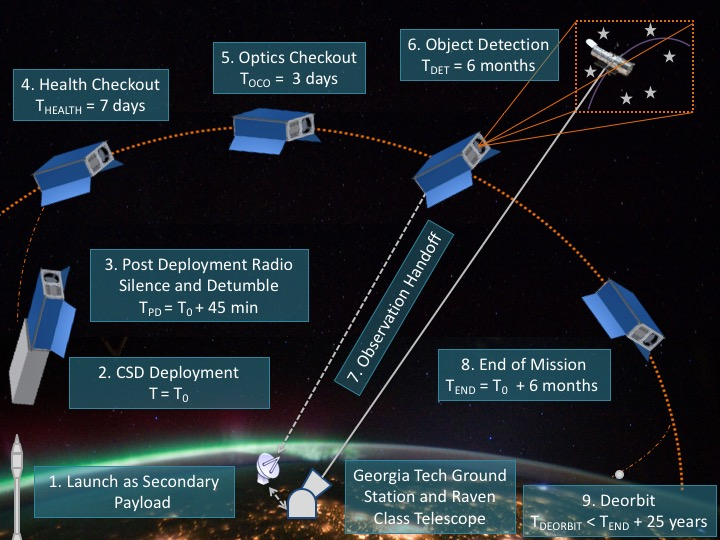
\includegraphics[width=.83\textwidth]{OV1.jpg}
\end{figure}

\begin{figure}[h!]
\centering
\caption{Operation of RECONSO over the course of a given orbit.}
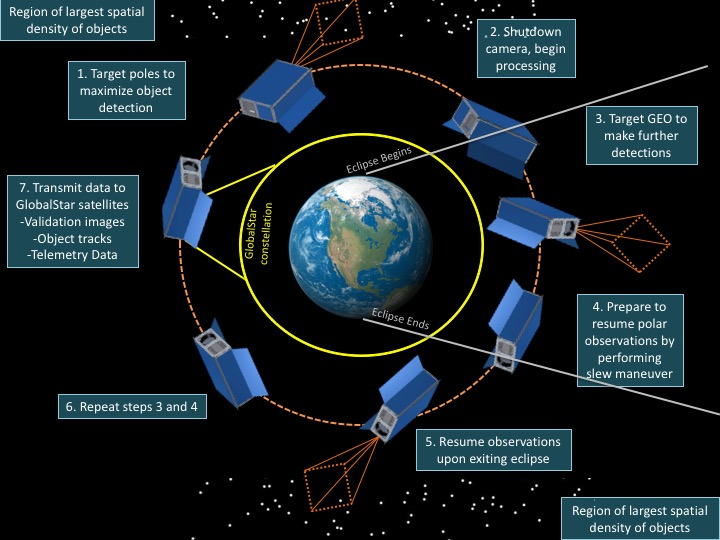
\includegraphics[width=.83\textwidth]{OV2.jpg}
\end{figure}

\newpage

In order to accomplish these operations, the satellite will have 13 modes of operation between which it will switch. The remainder of this document will be dedicated to addressing each of these modes in detail. The overview, entry criteria, exit criteria, operational hardware, and operational software of each mode will be described, along with any additional pertinent information that goes with each mode.

Before beginning, it should be noted that there are certain pieces of hardware and software that will always be used, throughout all modes of spacecraft operation. In the interest of avoiding repetitiveness, these items will be outlined in the table below. They will not be included in the tables defining the operational hardware and software in subsequent mode definitions.

\begin{table}[h!]
\caption{Operational components of the RECONSO system throughout all modes.}
\begin{adjustbox}{center}
\begin{tabular}{|l|l|}
\hline
Subsystem & Hardware \\ \hline \hline
EPS & ClydeSpace 30Whr Battery \\ \hline
EPS & ClydeSpace PMAD Distribution board  \\ \hline
EPS & In-house EPS Breakout board \\ \hline
EPS & In-house Inhibit board  \\ \hline
EPS & In-house Solar panels  \\ \hline \hline
AVI & Tyvak Intrepid \\ \hline
AVI & In-house CDH Breakout board \\ \hline 
\end{tabular}

\quad

\begin{tabular}{|l|l|}
\hline
Software & Processor \\ \hline \hline
Health Monitoring & Tyvak Intrepid \\ \hline
EPS Hardware Controller & Tyvak Intrepid \\ \hline
Finite State Machine (FSM) & Tyvak Intrepid \\ \hline
Scheduler & Tyvak Intrepid \\ \hline
File Manager & Tyvak Intrepid \\ \hline
Message Bus & Tyvak Intrepid \\ \hline
Event Log & Tyvak Intrepid \\ \hline
UHF COM Receive & Tyvak Intrepid \\ \hline
GlobalStar COM Receive & Tyvak Intrepid \\ \hline
\end{tabular}
\end{adjustbox}
\end{table}

It should be noted that the only items operational throughout all modes is only that hardware necessary to the integrity of the spacecraft. The EPS subsystem will always be conducting operations that help determine the health and basic functionality of the satellite. At it's most basic state, the batteries will be used to determine that an unacceptable depth of discharge has been reached and only the bare minimum hardware and software will be run until the batteries can be replenished through power output from the solar panels.

Each of the following subsections will list only hardware and software items that will be used \underline{\textbf{in addition}} to these items.

\newpage

\subsection{Post Deployment}

\underline{Overview:} There are no extra hardware or software items required of the satellite in this mode. The Post Deployment mode of operation will only be entered once throughout the mission lifetime. After being ejected from the CSD as a secondary payload, RECONSO will power on, but only with the bare minimum operation and no radio communications. This is a launch provider requirement so that the communications of secondary payloads do not interfere with communications between the ground and the primary payload or launch vehicle.

\underline{Entry Criteria:} 

\begin{enumerate}
\item Confirmation of launch vehicle ejection.
\end{enumerate}

\underline{Exit Criteria:} 

\begin{enumerate}
\item Passage of 45 minutes after launch vehicle ejection.
\end{enumerate}

\begin{table}[h!]
\caption{Additional components of RECONSO required for Post Deployment mode.}
\begin{adjustbox}{center}
\begin{tabular}{|l|l|}
\hline
Subsystem & Hardware \\ \hline \hline
None & None  \\ \hline
\end{tabular}

\quad

\begin{tabular}{|l|l|}
\hline
Software & Processor \\ \hline \hline
None & None \\ \hline
\end{tabular}
\end{adjustbox}
\end{table}

\newpage

\subsection{Detumble}

\underline{Overview:} The detumble mode will be used to null any unacceptably high angular rates and to return the spacecraft to a steady attitude. It will primarily be used directly after exiting the post deployment mode, when angular values are likely to be highest due to angular rates imparted by launch vehicle separation. It will also be used at any time throughout the mission when the Health Monitoring software determines that unacceptably high angular rates have been incurred. These rates could be imparted by anything from solar pressure to micrometeoroid impact. Once the angular rates have been nulled, the spacecraft will be placed into safe mode.

\underline{Entry Criteria:} 

\begin{enumerate}
\item Exit of Post Deployment mode
\item Unacceptably high angular rates
\end{enumerate}

\underline{Exit Criteria:}

\begin{enumerate}
\item Acceptably low angular rates
\end{enumerate}

\begin{table}[h!]
\caption{Additional components of RECONSO required for Detumble mode.}
\begin{adjustbox}{center}
\begin{tabular}{|l|l|}
\hline
Subsystem & Hardware \\ \hline \hline
ADCS & Analog Devices Inertial Measurement Unit  \\ \hline
ADCS & In-house sun sensors  \\ \hline
ADCS & In-house magnetorquers  \\ \hline
ADCS & Tyvak Magnetometer \\ \hline
ADCS & BBB ADCS Controller \\ \hline
\end{tabular}

\quad

\begin{tabular}{|l|l|}
\hline
Software & Processor \\ \hline \hline
ADCS Controller & BBB \\ \hline
ADCS Hardware polling & BBB \\ \hline \hline
BBB Hardware Controller & Tyvak Intrepid \\ \hline
\end{tabular}
\end{adjustbox}
\end{table}

\newpage

\subsection{Safe Mode}

\underline{Overview:} Safe mode is designed to be the bare minimum operations that the spacecraft can carry out. It will be placed into this mode upon a reboot of the primary flight computer and at any time throughout spacecraft operations that a health measurement is recorded outside of nominal bounds for a given component, as specified in Appendix B. If the health monitoring code detects unacceptable health values, it will kill any active processes and record in the Event Log the reasoning for entering safe mode. Telemetry will be polled and recorded throughout safe mode operation so that it can be determined when the system is ready to exit safe mode. COM will be enabled during this mode so that the ground can understand why the spacecraft has entered this mode and any changes to the planned operations can be made. Only UHF COM will be utilized in safe mode in order to maximize the power efficiency and protect the battery from critical levels. Fine pointing will not be required as the mostly omnidirectional nature of the UHF COM systems will allow for low-throughput communications that will be required for the ground to accurately diagnose the situation and command any basic operation that will bring the spacecraft out of safe mode. The ADCS and TCS subsystems remain active throughout safe mode to ensure the payload lens remains healthy and does not point directly at the sun or exceed a nominal temperature range.

It should also be noted that every other mode of operation has exit criteria equivalent to the entry criteria of safe mode, i.e. if any of the anomalies that trigger safe mode occur in any other operating mode, that mode is terminated and safe mode is initiated.

\underline{Entry Criteria:} 

\begin{enumerate}
\item Temperatures higher than 50 \degree C
\item Temperatures lower than -10 \degree C
\item Unacceptable power draw
\item Detection of more than 80\% depth of discharge
\item Detection of voltage spike
\end{enumerate}

\underline{Exit Criteria:}

\begin{enumerate}
\item Nominal health readings 
\item Ground station receipt of all telemetry leading up to triggering of safe mode
\item Ground station receipt of healthy telemetry after occurrence of anomaly
\item Ground station confirmation that satellite is capable of returning to nominal operation
\end{enumerate}

\begin{table}[h!]
\caption{Additional components of RECONSO required for Safe mode.}
\begin{adjustbox}{center}
\begin{tabular}{|l|l|}
\hline
Subsystem & Hardware \\ \hline \hline
ADCS & Analog Devices Inertial Measurement Unit  \\ \hline
ADCS & Pumpkin GPSRM 1 GPS Receiver \\ \hline
ADCS & AntCom 1.5G L1 GPS Antenna  \\ \hline
ADCS & In-house sun sensors  \\ \hline
ADCS & In-house magnetorquers  \\ \hline
ADCS & Tyvak Magnetometer \\ \hline
ADCS & BBB ADCS Controller \\ \hline \hline
COM & Tyvak UHF Daughterboard  \\ \hline
COM & ISIS UHF Dipole Antenna  \\ \hline
%COM & NSL GlobalStar Duplex  \\ \hline
%COM & NSL GlobalStar Patch Antenna \\ \hline \hline
TCS & Omega Resistive Temperature Detector \\ \hline
TCS & Omega 10 Whr Heater  \\ \hline
TCS & In-house thermal board \\ \hline
\end{tabular}

\quad

\begin{tabular}{|l|l|}
\hline
Software & Processor \\ \hline \hline
ADCS Controller & BBB \\ \hline
ADCS Hardware polling & BBB \\ \hline \hline
TCS Hardware Controller & Tyvak Intrepid \\ \hline
BBB Hardware Controller & Tyvak Intrepid \\ \hline
UHF COM Receive & Tyvak Intrepid \\ \hline
UHF COM Transmit & Tyvak Intrepid \\ \hline
GlobalStar COM Receive & Tyvak Intrepid \\ \hline
GlobalStar COM Transmit & Tyvak Intrepid \\ \hline
\end{tabular}
\end{adjustbox}
\end{table}

\newpage

\subsection{Systems Checkouts}

\underline{Overview:} The Systems Checkouts mode will be used for diagnosing the long term health of the spacecraft. As such, it varies from Safe mode only slightly. Systems Checkouts will be used at two different times throughout the lifecycle of the spacecraft: upon exiting safe mode for the first time after launch and upon ground station commanding of this mode. Upon first exiting safe mode, the spacecraft will remain in this mode for 7 days. This will be done to determine that there has not been any subtle degradation of the spacecraft hardware cause by the launch environment and that it is able to function for extended periods of time. During this mode, telemetry will be sent from the spacecraft down to the ground station every hour in the form of a beacon. To ensure the health of GlobalStar system, this beacon will first be sent over GlobalStar COM. However, in order to ensure that the UHF COM is also functional, the ground station will command the satellite to switch to UHF after verifying health of the GlobalStar system. This will allow for proper testing of both COM systems and allow the mission operations team to address any problems with the spacecraft before they become untenable. The spacecraft will exit this mode of operation when commanded to do so by the ground station.

\underline{Entry Criteria:} 

\begin{enumerate}
\item First exit of safe mode
\item Commanding by ground station
\end{enumerate}

\underline{Exit Criteria:}

\begin{enumerate}
\item Commanding by ground station
\end{enumerate}

\begin{table}[h!]
\caption{Additional components of RECONSO required for Systems Checkouts mode.}
\begin{adjustbox}{center}
\begin{tabular}{|l|l|}
\hline
Subsystem & Hardware \\ \hline \hline
ADCS & Analog Devices Inertial Measurement Unit  \\ \hline
ADCS & Pumpkin GPSRM 1 GPS Receiver \\ \hline
ADCS & AntCom 1.5G L1 GPS Antenna  \\ \hline
ADCS & In-house sun sensors  \\ \hline
ADCS & In-house magnetorquers  \\ \hline
ADCS & Tyvak Magnetometer \\ \hline
ADCS & BBB ADCS Controller \\ \hline \hline
% COM & Tyvak UHF Daughterboard  \\ \hline
COM & ISIS UHF Dipole Antenna  \\ \hline
COM & NSL GlobalStar Duplex  \\ \hline
COM & NSL GlobalStar Patch Antenna \\ \hline \hline
TCS & Omega Resistive Temperature Detector \\ \hline
TCS & Omega 10 Whr Heater  \\ \hline
TCS & In-house thermal board \\ \hline
\end{tabular}

\quad

\begin{tabular}{|l|l|}
\hline
Software & Processor \\ \hline \hline
ADCS Controller & BBB \\ \hline
ADCS Hardware polling & BBB \\ \hline \hline
TCS Hardware Controller & Tyvak Intrepid \\ \hline
BBB Hardware Controller & Tyvak Intrepid \\ \hline
UHF COM Receive & Tyvak Intrepid \\ \hline
UHF COM Transmit & Tyvak Intrepid \\ \hline
GlobalStar COM Receive & Tyvak Intrepid \\ \hline
GlobalStar COM Transmit & Tyvak Intrepid \\ \hline
\end{tabular}
\end{adjustbox}
\end{table}

\newpage

\subsection{Optics Checkouts}

\underline{Overview:} Similar to Systems Checkouts, Optics Checkouts will be entered immediately upon the first exiting of Systems Checkouts mode or upon commanding by the ground station. This mode is designed to test the integrity of the mission payload by taking a series of images and downlinking them to the ground. The ground will command mission times and pointing commands at which the spacecraft should take an image, and the spacecraft will do so. This will allow further integrated testing of on-orbit performance necessary for nominal operations and will again allow the spacecraft operators to understand any foibles or errors in the spacecraft functionality before nominal operations commence. A minimum of 1 validation image will be downlinked, but more may be requested should the first be deemed insufficient to make a confident decision. Star tracking will also be demonstrated in this mode and the resultant telemetry will be downlinked along with the validation image.

\underline{Entry Criteria:} 

\begin{enumerate}
\item First exit of Systems Checkouts Mode
\item Commanding by ground station
\end{enumerate}

\underline{Exit Criteria:}

\begin{enumerate}
\item Commanding by ground station
\end{enumerate}

\begin{table}[h!]
\caption{Additional components of RECONSO required for Optics Checkouts mode.}
\begin{adjustbox}{center}
\begin{tabular}{|l|l|}
\hline
Subsystem & Hardware \\ \hline \hline
PAY & Nocturn 50mm f/0.95 Lens  \\ \hline
PAY & Nocturn XL CMOS Camera  \\ \hline
PAY & Innoflight CFC-300 Processor  \\ \hline \hline
ADCS & Analog Devices Inertial Measurement Unit  \\ \hline
ADCS & Pumpkin GPSRM 1 GPS Receiver \\ \hline
ADCS & AntCom 1.5G L1 GPS Antenna  \\ \hline
ADCS & In-house sun sensors  \\ \hline
ADCS & In-house magnetorquers  \\ \hline
ADCS & Tyvak Magnetometer \\ \hline
ADCS & BBB ADCS Controller \\ \hline \hline
% COM & Tyvak UHF Daughterboard  \\ \hline
COM & ISIS UHF Dipole Antenna  \\ \hline
COM & NSL GlobalStar Duplex  \\ \hline
COM & NSL GlobalStar Patch Antenna \\ \hline \hline
TCS & Omega Resistive Temperature Detector \\ \hline
TCS & Omega 10 Whr Heater  \\ \hline
TCS & In-house thermal board \\ \hline
\end{tabular}

\quad

\begin{tabular}{|l|l|}
\hline
Software & Processor \\ \hline \hline
Image Processing & CFC-300 \\ \hline
Star Tracker & CFC-300 \\ \hline
ADCS Controller & BBB \\ \hline
ADCS Hardware polling & BBB \\ \hline \hline
TCS Hardware Controller & Tyvak Intrepid \\ \hline
Innoflight CFC-300 Hardware Controller & Tyvak Intrepid \\ \hline
BBB Hardware Controller & Tyvak Intrepid \\ \hline
UHF COM Receive & Tyvak Intrepid \\ \hline
UHF COM Transmit & Tyvak Intrepid \\ \hline
GlobalStar COM Receive & Tyvak Intrepid \\ \hline
GlobalStar COM Transmit & Tyvak Intrepid \\ \hline
\end{tabular}
\end{adjustbox}
\end{table}

\newpage

\subsection{Sunlight Operations}

\underline{Overview:} The Sunlight Operations mode will be the only mode in which the spacecraft gathers relevant mission data. This mode will be entered once the spacecraft has arrived at a location in its orbit where it needs to gather data (either polar region or approach to the equator), is pointing at the correct attitude to gather data, has determined that it has sufficient disk space to write payload images, and is completely healthy. The spacecraft will then take images at a frequency of 10 Hz until it has passed through the region in which it needed to gather data. While it is taking these images, star tracking will be employed to determine the attitude of the spacecraft. Each image will also be time-tagged so that later analysis can correlate tracks to GPS locations and attitude states.

\underline{Entry Criteria:} 

\begin{enumerate}
\item Arrival in region of payload operation
\item Correct execution of pointing command
\item Sufficient disk space for payload operation
\item Nominal health
\end{enumerate}

\underline{Exit Criteria:}

\begin{enumerate}
\item Exit from region of payload operation
\end{enumerate}

\begin{table}[h!]
\caption{Additional components of RECONSO required for Sunlight Operations mode.}
\begin{adjustbox}{center}
\begin{tabular}{|l|l|}
\hline
Subsystem & Hardware \\ \hline \hline
PAY & Nocturn 50mm f/0.95 Lens  \\ \hline
PAY & Nocturn XL CMOS Camera  \\ \hline
PAY & Innoflight CFC-300 Processor  \\ \hline \hline
ADCS & Analog Devices Inertial Measurement Unit  \\ \hline
ADCS & Pumpkin GPSRM 1 GPS Receiver \\ \hline
ADCS & AntCom 1.5G L1 GPS Antenna  \\ \hline
ADCS & In-house sun sensors  \\ \hline
ADCS & Tyvak Magnetometer \\ \hline
ADCS & BBB ADCS Controller \\ \hline \hline
% COM & Tyvak UHF Daughterboard  \\ \hline
COM & ISIS UHF Dipole Antenna  \\ \hline
COM & NSL GlobalStar Duplex  \\ \hline
COM & NSL GlobalStar Patch Antenna \\ \hline \hline
TCS & Omega Resistive Temperature Detector \\ \hline
TCS & Omega 10 Whr Heater  \\ \hline
TCS & In-house thermal board \\ \hline
\end{tabular}

\quad

\begin{tabular}{|l|l|}
\hline
Software & Processor \\ \hline \hline
Image Processing & CFC-300 \\ \hline
Star Tracker & CFC-300 \\ \hline
Star Subtraction & CFC-300 \\ \hline
Object Tracking & CFC-300 \\ \hline \hline
ADCS Controller & BBB \\ \hline
ADCS Hardware polling & BBB \\ \hline \hline
TCS Hardware Controller & Tyvak Intrepid \\ \hline
Innoflight CFC-300 Hardware Controller & Tyvak Intrepid \\ \hline
BBB Hardware Controller & Tyvak Intrepid \\ \hline
UHF COM Receive & Tyvak Intrepid \\ \hline
GlobalStar COM Receive & Tyvak Intrepid \\ \hline
\end{tabular}
\end{adjustbox}
\end{table}

\newpage

\subsection{Sunlight Data Processing}

\underline{Overview:} If, in evaluating the entry conditions for entrance of Sunlight Operations mode, there is insufficient disk space on the CFC-300 to write images, the spacecraft will instead enter Sunlight Data Processing mode. In this case, the spacecraft will process the images remaining in memory and create a data product, rather than take new images. After completing this process, the spacecraft will enter Sunlight Nominal mode.

\underline{Entry Criteria:} 

\begin{enumerate}
\item Arrival in region of payload operation
\item Correct execution of pointing command
\item \textbf{In}sufficient disk space for payload operation
\item Nominal health
\end{enumerate}

\underline{Exit Criteria:}

\begin{enumerate}
\item Sufficient disk space for payload operation
\end{enumerate}

\begin{table}[h!]
\caption{Additional components of RECONSO required for Sunlight Data Processing mode.}
\begin{adjustbox}{center}
\begin{tabular}{|l|l|}
\hline
Subsystem & Hardware \\ \hline \hline
ADCS & Analog Devices Inertial Measurement Unit  \\ \hline
ADCS & Pumpkin GPSRM 1 GPS Receiver \\ \hline
ADCS & AntCom 1.5G L1 GPS Antenna  \\ \hline
ADCS & In-house sun sensors  \\ \hline
ADCS & Tyvak Magnetometer \\ \hline
ADCS & BBB ADCS Controller \\ \hline \hline
% COM & Tyvak UHF Daughterboard  \\ \hline
COM & ISIS UHF Dipole Antenna  \\ \hline
COM & NSL GlobalStar Duplex  \\ \hline
COM & NSL GlobalStar Patch Antenna \\ \hline \hline
TCS & Omega Resistive Temperature Detector \\ \hline
TCS & Omega 10 Whr Heater  \\ \hline
TCS & In-house thermal board \\ \hline
\end{tabular}

\quad

\begin{tabular}{|l|l|}
\hline
Software & Processor \\ \hline \hline
Image Processing & CFC-300 \\ \hline
Star Tracker & CFC-300 \\ \hline
Star Subtraction & CFC-300 \\ \hline
Object Tracking & CFC-300 \\ \hline \hline
ADCS Controller & BBB \\ \hline
ADCS Hardware polling & BBB \\ \hline \hline
TCS Hardware Controller & Tyvak Intrepid \\ \hline
Innoflight CFC-300 Hardware Controller & Tyvak Intrepid \\ \hline
BBB Hardware Controller & Tyvak Intrepid \\ \hline
UHF COM Receive & Tyvak Intrepid \\ \hline
GlobalStar COM Receive & Tyvak Intrepid \\ \hline
\end{tabular}
\end{adjustbox}
\end{table}

\newpage

\subsection{Sunlight Transmit}

\underline{Overview:} Given the quasi-global coverage supplied by the GlobalStar network, the transmission of data from the spacecraft to the ground can occur at any point in the spacecraft's orbit. As such, the spacecraft will, at a minimum enter this mode to downlink health data to the ground. If the spacecraft has made one of more tracks since last entering transmit mode, those tracks will be downlinked as well. Should the spacecraft not register any tracks after data processing, only health data will be downlinked and the FSM will direct the spacecraft straight to Sunlight Nominal Operations. Given that the spacecraft will constantly be able to receive messages while outside of Post Deployment mode, this mode will also be entered should the ground command a response from the spacecraft.

\underline{Entry Criteria:} 

\begin{enumerate}
\item Completion of Sunlight Data Processing
\item Commanding by ground station
\end{enumerate}

\underline{Exit Criteria:}

\begin{enumerate}
\item Completion of transmission
\end{enumerate}

\begin{table}[h!]
\caption{Additional components of RECONSO required for Sunlight Transmit mode.}
\begin{adjustbox}{center}
\begin{tabular}{|l|l|}
\hline
Subsystem & Hardware \\ \hline \hline
PAY & Innoflight CFC-300 Processor  \\ \hline \hline
ADCS & Analog Devices Inertial Measurement Unit  \\ \hline
ADCS & Pumpkin GPSRM 1 GPS Receiver \\ \hline
ADCS & AntCom 1.5G L1 GPS Antenna  \\ \hline
ADCS & In-house sun sensors  \\ \hline
ADCS & Tyvak Magnetometer \\ \hline
ADCS & BBB ADCS Controller \\ \hline \hline
% COM & Tyvak UHF Daughterboard  \\ \hline
COM & ISIS UHF Dipole Antenna  \\ \hline
COM & NSL GlobalStar Duplex  \\ \hline
COM & NSL GlobalStar Patch Antenna \\ \hline \hline
TCS & Omega Resistive Temperature Detector \\ \hline
TCS & Omega 10 Whr Heater  \\ \hline
TCS & In-house thermal board \\ \hline
\end{tabular}

\quad

\begin{tabular}{|l|l|}
\hline
Software & Processor \\ \hline \hline
ADCS Controller & BBB \\ \hline
ADCS Hardware polling & BBB \\ \hline \hline
TCS Hardware Controller & Tyvak Intrepid \\ \hline
Innoflight CFC-300 Hardware Controller & Tyvak Intrepid \\ \hline
BBB Hardware Controller & Tyvak Intrepid \\ \hline
UHF COM Receive & Tyvak Intrepid \\ \hline
UHF COM Transmit & Tyvak Intrepid \\ \hline
GlobalStar COM Receive & Tyvak Intrepid \\ \hline
GlobalStar COM Transmit & Tyvak Intrepid \\ \hline
\end{tabular}
\end{adjustbox}
\end{table}

\newpage

\subsection{Sunlight Nominal}

\underline{Overview:} The Sunlight Nominal mode will be entered once the Sunlight Transmit mode is completed, but while the satellite is still in sunlight and is generating power. During this time, the spacecraft will make any attitude adjustments necessary for the next phase of operations (either a polar or equatorial region) and then wait until it is passes into a region suitable for those operations.

\underline{Entry Criteria:} 

\begin{enumerate}
\item Exit from Sunlight Transmit or Sunlight Data Processing modes
\end{enumerate}

\underline{Exit Criteria:}

\begin{enumerate}
\item Accomplishment of next pointing command
\item Entrance into eclipse
\end{enumerate}

\begin{table}[h!]
\caption{Additional components of RECONSO required for Sunlight Nominal mode.}
\begin{adjustbox}{center}
\begin{tabular}{|l|l|}
\hline
Subsystem & Hardware \\ \hline \hline
ADCS & Analog Devices Inertial Measurement Unit  \\ \hline
ADCS & Pumpkin GPSRM 1 GPS Receiver \\ \hline
ADCS & AntCom 1.5G L1 GPS Antenna  \\ \hline
ADCS & In-house sun sensors  \\ \hline
ADCS & Tyvak Magnetometer \\ \hline
ADCS & In-house magnetorquers \\ \hline
ADCS & BBB ADCS Controller \\ \hline \hline
% COM & Tyvak UHF Daughterboard  \\ \hline
COM & ISIS UHF Dipole Antenna  \\ \hline
COM & NSL GlobalStar Duplex  \\ \hline
COM & NSL GlobalStar Patch Antenna \\ \hline \hline
TCS & Omega Resistive Temperature Detector \\ \hline
TCS & Omega 10 Whr Heater  \\ \hline
TCS & In-house thermal board \\ \hline
\end{tabular}

\quad

\begin{tabular}{|l|l|}
\hline
Software & Processor \\ \hline \hline
ADCS Controller & BBB \\ \hline
ADCS Hardware polling & BBB \\ \hline \hline
TCS Hardware Controller & Tyvak Intrepid \\ \hline
Innoflight CFC-300 Hardware Controller & Tyvak Intrepid \\ \hline
BBB Hardware Controller & Tyvak Intrepid \\ \hline
UHF COM Receive & Tyvak Intrepid \\ \hline
GlobalStar COM Receive & Tyvak Intrepid \\ \hline
\end{tabular}
\end{adjustbox}
\end{table}

\newpage

\subsection{Eclipse Data Processing}

\underline{Overview:} The Eclipse Data Processing mode is very similar to Sunlight Data Processing in that it processes whatever is left of the payload image data after it has been gathered and saved to disk. However, there is a difference in hardware used during this mode as the spacecraft should be in a lower power state while in eclipse so as not reach an unacceptable depth of discharge. In addition, due to the heavy power requirement of the Innoflight CFC-300 hardware, this state must be entered by command from the ground station upon verification that there is a sufficient battery charge remaining.

It is assumed that the spacecraft will not be collecting data while it is in eclipse, so if there is no data to be processed, this mode will not be entered.

\underline{Entry Criteria:} 

\begin{enumerate}
\item Entrance into eclipse
\item Unprocessed payload data still on disk
\item Command from ground station after verification of sufficient battery charge
\end{enumerate}

\underline{Exit Criteria:}

\begin{enumerate}
\item Exit of eclipse or finishing of data processing, whichever comes first.
\end{enumerate}

\begin{table}[h!]
\caption{Additional components of RECONSO required for Eclipse Data Processing mode.}
\begin{adjustbox}{center}
\begin{tabular}{|l|l|}
\hline
Subsystem & Hardware \\ \hline \hline
PAY & Innoflight CFC-300 Processor  \\ \hline \hline
ADCS & In-house sun sensors  \\ \hline
ADCS & Tyvak Magnetometer \\ \hline
ADCS & BBB ADCS Controller \\ \hline \hline
% COM & Tyvak UHF Daughterboard  \\ \hline
COM & ISIS UHF Dipole Antenna  \\ \hline
COM & NSL GlobalStar Duplex  \\ \hline
COM & NSL GlobalStar Patch Antenna \\ \hline \hline
TCS & Omega Resistive Temperature Detector \\ \hline
TCS & Omega 10 Whr Heater  \\ \hline
TCS & In-house thermal board \\ \hline
\end{tabular}

\quad

\begin{tabular}{|l|l|}
\hline
Software & Processor \\ \hline \hline
Image Processing & CFC-300 \\ \hline
Star Subtraction & CFC-300 \\ \hline
Object Tracking & CFC-300 \\ \hline \hline
ADCS Controller & BBB \\ \hline
ADCS Hardware polling & BBB \\ \hline \hline
TCS Hardware Controller & Tyvak Intrepid \\ \hline
Innoflight CFC-300 Hardware Controller & Tyvak Intrepid \\ \hline
BBB Hardware Controller & Tyvak Intrepid \\ \hline
UHF COM Receive & Tyvak Intrepid \\ \hline
GlobalStar COM Receive & Tyvak Intrepid \\ \hline
\end{tabular}
\end{adjustbox}
\end{table}

\newpage

\subsection{Eclipse Transmit}

\underline{Overview:} Much like Sunlight Transmit mode, Eclipse Transmit will occur if, once data processing has completed, there is payload data that has not been downlinked to the ground. However, it differs from Sunlight Transmit in that, it will not downlink telemetry unless commanded by the ground station to do so. Due to the high power requirements of transmission, it is desirable to limit transmission time while in eclipse as much as is possible. Once all necessary data has been transmitted, RECONSO will exit this mode.

\underline{Entry Criteria:} 

\begin{enumerate}
\item Completion of Eclipse Data Processing
\item Payload data on disk that has not been downlinked
\item Command from ground station after verification of sufficient battery charge
\end{enumerate}

\underline{Exit Criteria:}

\begin{enumerate}
\item Completion of transmission or lack thereof
\end{enumerate}

\begin{table}[h!]
\caption{Additional components of RECONSO required for Eclipse Transmit mode.}
\begin{adjustbox}{center}
\begin{tabular}{|l|l|}
\hline
Subsystem & Hardware \\ \hline \hline
PAY & Innoflight CFC-300 Processor  \\ \hline \hline
ADCS & In-house sun sensors  \\ \hline
ADCS & Tyvak Magnetometer \\ \hline
ADCS & BBB ADCS Controller \\ \hline \hline
% COM & Tyvak UHF Daughterboard  \\ \hline
COM & ISIS UHF Dipole Antenna  \\ \hline
COM & NSL GlobalStar Duplex  \\ \hline
COM & NSL GlobalStar Patch Antenna \\ \hline \hline
TCS & Omega Resistive Temperature Detector \\ \hline
TCS & Omega 10 Whr Heater  \\ \hline
TCS & In-house thermal board \\ \hline
\end{tabular}

\quad

\begin{tabular}{|l|l|}
\hline
Software & Processor \\ \hline \hline
Image Processing & CFC-300 \\ \hline
Star Subtraction & CFC-300 \\ \hline
Object Tracking & CFC-300 \\ \hline \hline
ADCS Controller & BBB \\ \hline
ADCS Hardware polling & BBB \\ \hline \hline
TCS Hardware Controller & Tyvak Intrepid \\ \hline
Innoflight CFC-300 Hardware Controller & Tyvak Intrepid \\ \hline
BBB Hardware Controller & Tyvak Intrepid \\ \hline
UHF COM Receive & Tyvak Intrepid \\ \hline
UHF COM Transmit & Tyvak Intrepid \\ \hline
GlobalStar COM Receive & Tyvak Intrepid \\ \hline
GlobalStar COM Transmit & Tyvak Intrepid \\ \hline
\end{tabular}
\end{adjustbox}
\end{table}

\newpage

\subsection{Eclipse Nominal}

\underline{Overview:} Upon completion of Eclipse Transmit mode or Eclipse Data Processing mode (or having never entered either), the spacecraft will enter Eclipse Nominal mode. Upon verification of a sufficient battery charge, the next pointing command relevant to the gathering of payload data will be executed. Given that the spacecraft is in eclipse, this will be towards one of the poles as opposed to towards the equator. Upon completing this slew maneuver, the spacecraft will wait until entering sunlight and further payload operations.

If the battery charge level is deemed insufficient to avoid entering safe mode due to depth of discharge, this state will not execute a pointing command and therefore idle until the end of eclipse.

\underline{Entry Criteria:} 

\begin{enumerate}
\item Completion of Eclipse Transmit
\end{enumerate}

\underline{Exit Criteria:}

\begin{enumerate}
\item Accomplishment of next pointing command
\item Entrance into sunlight
\item Pointing command executed upon verification of sufficient battery power remaining
\end{enumerate}

\begin{table}[h!]
\caption{Additional components of RECONSO required for Eclipse Nominal mode.}
\begin{adjustbox}{center}
\begin{tabular}{|l|l|}
\hline
Subsystem & Hardware \\ \hline \hline
ADCS & In-house sun sensors  \\ \hline
ADCS & Tyvak Magnetometer \\ \hline
ADCS & BBB ADCS Controller \\ \hline \hline
% COM & Tyvak UHF Daughterboard  \\ \hline
COM & ISIS UHF Dipole Antenna  \\ \hline
COM & NSL GlobalStar Duplex  \\ \hline
COM & NSL GlobalStar Patch Antenna \\ \hline \hline
TCS & Omega Resistive Temperature Detector \\ \hline
TCS & Omega 10 Whr Heater  \\ \hline
TCS & In-house thermal board \\ \hline
\end{tabular}

\quad

\begin{tabular}{|l|l|}
\hline
Software & Processor \\ \hline \hline
ADCS Controller & BBB \\ \hline
ADCS Hardware polling & BBB \\ \hline \hline
TCS Hardware Controller & Tyvak Intrepid \\ \hline
BBB Hardware Controller & Tyvak Intrepid \\ \hline
UHF COM Receive & Tyvak Intrepid \\ \hline
GlobalStar COM Receive & Tyvak Intrepid \\ \hline
\end{tabular}
\end{adjustbox}
\end{table}

\newpage

\subsection{End of Life}

\underline{Overview:} After a mission lifetime of 6 months or upon incurring a fatal hardware error, the spacecraft will be put into End of Life mode. The goal of the End of Life mode is to ensure that the spacecraft does not transmit or receive on any frequencies while it safely de-orbits within the 25 year limit. Given that RECONSO is employing solely passive de-orbit procedures, there is a possibility that this mode will last for quite a long time. The ground station will command a series of commands the spacecraft that will allow it to shut down without the aid of the ground station. The commands will be as follows: put the satellite into safe mode, command the PMAD to shunt all power generated by the solar panels, turn off the flight computer. This will eventually drain the batteries without leaving them a possibility or recharging, and RECONSO will die a natural death. 

It should be noted that while COM hardware and software is listed as being necessary for this mode, it is only necessary for the entrance to this mode. It will not be operation while within End of Life mode. Should all COM hardware be anomalous, the end goal of this mode will have already been accomplished and thus will not be necessary.

\underline{Entry Criteria:} 

\begin{enumerate}
\item Commanding by ground station
\end{enumerate}

\underline{Exit Criteria:}

\begin{enumerate}
\item None
\end{enumerate}

\begin{table}[h!]
\caption{Additional components of RECONSO required for End of Life mode.}
\begin{adjustbox}{center}
\begin{tabular}{|l|l|}
\hline
Subsystem & Hardware \\ \hline \hline
% COM & Tyvak UHF Daughterboard  \\ \hline
COM & ISIS UHF Dipole Antenna  \\ \hline
COM & NSL GlobalStar Duplex  \\ \hline
COM & NSL GlobalStar Patch Antenna \\ \hline
\end{tabular}

\quad

\begin{tabular}{|l|l|}
\hline
Software & Processor \\ \hline \hline
UHF COM Receive & Tyvak Intrepid \\ \hline
GlobalStar COM Receive & Tyvak Intrepid \\ \hline
\end{tabular}
\end{adjustbox}
\end{table}

\section{Conclusion}

There are a total of 13 modes of operation of RECONSO, each accomplishing a unique function. To reiterate, the FSM code will handle all switching between each mode autonomously based on pre-defined entry an exit criteria. Once the nominal mission lifetime of RECONSO has been accomplished, the End of Life mode will be commanded, and the mission will be permanently ended. Please reference Appendix A for a visual flow chart representation of this same information.

\newpage

\section{Appendix A: \\ Mode Switching Flow Chart}

Note: This image is best viewed in a digital format, where the reader can zoom in on any desired section of the flow chart.

\begin{figure}[h!]
\centering
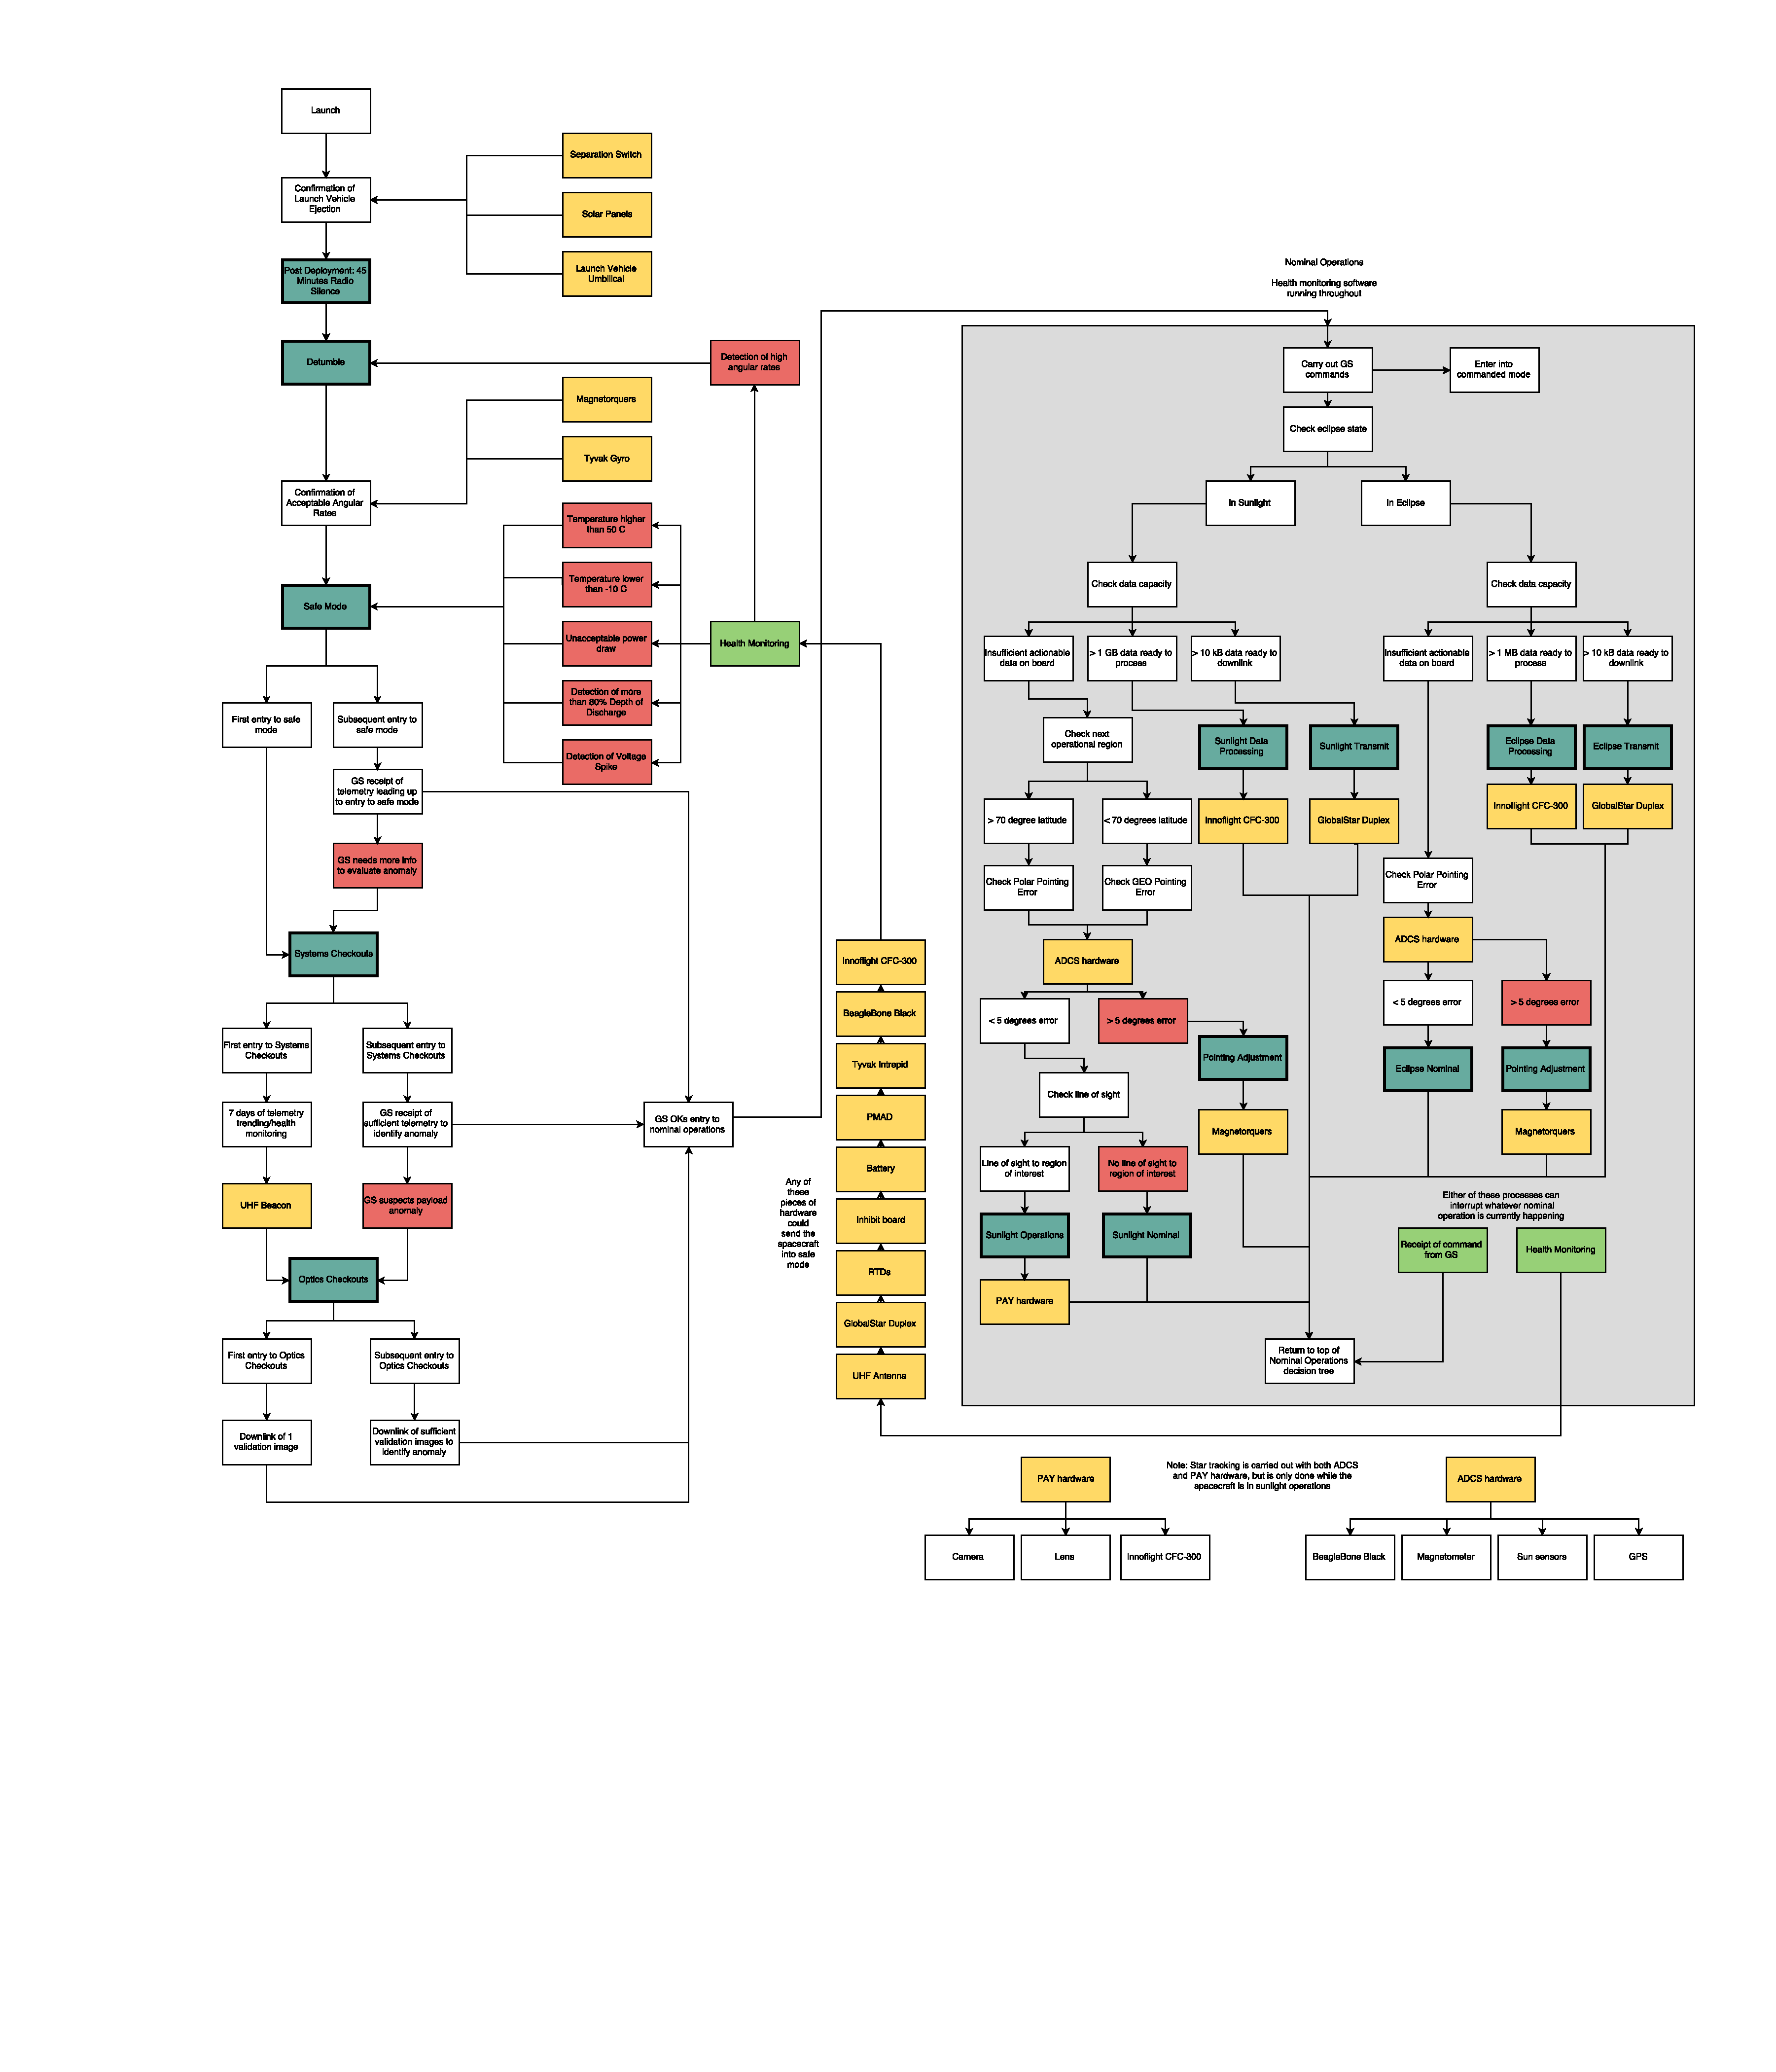
\includegraphics[width=\textwidth,height=.8\textheight]{FlowChart.pdf}
\end{figure} 

\newpage
\section{Appendix B: \\ Commands and Nominal Telemetry Values}

\begin{tabular}{|l|l|}
	\hline
	ADCS Commands      &  Nominal Result                \\ \hhline{|=|=|}
	ADCS_Telemetry GET_ADCS_TEL() & See specific telemetry points below \\ \hline
	float* MAGTORQ_CUR_CMD() & -0.3 to 0.3 \\ \hline
	float* V_ECI() & -1000 to 1000 \\ \hline
	float* Q_ECI_TO_BODY() & -7.67 to 7.67 \\ \hline
	float* ANGVEL_BODY() & -1 to 1 \\ \hline
	float VAR_ECI_POS() & -250 to 250 tumbling, -10 to 10 nominal \\ \hline
	float VAR_ECI_VEL() & TBD \\ \hline
	float VAR_BORESIGHT_ATTITUDE() & TBD \\ \hline
	uint8_t POINTINGMODE() & 1, 2, 3 ,4 \\ \hline
	float Q_ERROR_NORM() & 0 to 30 \\ \hline
	uint8_t SUNSENSOR_FLAG() & 0 or 1 \\ \hline
	uint8_t MAGMETER_FLAG() & 0 or 1  \\ \hline
	uint8_t FILTER_RESET_FLAG() & 0 or 1 \\ \hline
	uint16_t FILTER_RESET_TIMESTAMP() & Time \\ \hline
	float* GYRO_GYROFRAME_MEAS() & -250 to 250 tumbling, -10 to 10 nominal \\ \hline
	float* MAGMETER_MAGMETERFRAME_MEAS() & TBD \\ \hline
	float* ACCELMETER_ACCELMETERFRAME_MEAS() & TBD \\ \hline
	float* STARTRACKER_ECI_TO_BODY_MEAS() & 0 to 1 \\ \hline
	double GPS_DATA() & TBD \\ \hline
	float* SUNSENSOR_MEAS() & TBD \\ \hline
	TORQUE_ROD_X_CURRENT(float xcurr) & -0.3 to 0.3 \\ \hline
	TORQUE_ROD_Y_CURRENT(float ycurr) & -0.3 to 0.3 \\ \hline
	TORQUE_ROD_Z_CURRENT(float zcurr)  & -0.3 to 0.3 \\ \hline
	ADCS_Ack UPDATE_CONTROLLER_GAINS() & TBD \\ \hline
	ADCS_Ack UPLOAD_POINTING_PROFILE(uint8_t pprof) & 0 or 1 \\ \hline
	ADCS_Ack RESET_FILTER(uint8_t reset) & 0 or 1 \\ \hline
	ADCS_Ack SET_POINTING_MODE(uint8_t pmode) & 0, 1, 2, $\dots$, 5, 6 \\ \hline
	ADCS_Ack SET_AD_SENSORS(uint8_t adsensors) & 0, 1, 2, $\dots$, 9, 10 \\ \hline
\end{tabular}
\newpage
\begin{tabular}{|l|l|}
	\hline
	CDH Commands      &  Nominal Result                \\ \hhline{|=|=|}
	CDH_Telemetry GET_CDH_TEL() & See specific telemetry points below \\ \hline
	uint32_t TYV_CPU_USERTIME(void) & time \\ \hline
	uint32_t TYV_CPU_NICETIME(void) & time \\ \hline
	uint32_t TYV_SYS_TIME(void) & time \\ \hline
	uint32_t TYV_IDLE_TIME(void) & time \\ \hline
	uint32_t TYV_VIRT_PG_IN(void) & 0 to TBD \\ \hline
	uint32_t TYV_VIRT_PG_OUT(void) & 0 to TBD \\ \hline
	uint32_t TYV_PG_SWPS_IN_MEM(void) & 0 to TBD \\ \hline
	uint32_t TYV_PG_SWPS_OUT_MEM(void) & 0 to TBD \\ \hline
	uint32_t TYV_NUM_INTERUPTS(void) & 0 to TBD \\ \hline
	uint32_t TYV_NUM_PROC_CONTEXT_SWPS(void) & 0 to TBD \\ \hline
	uint32_t TYV_TIME_FROM_BOOT(void) & time \\ \hline
	uint32_t TYV_TOTAL_PROCESSES(void) & 0 to TBD \\ \hline
	uint32_t TYV_RUN_PROCESSES(void) & 0 to TBD \\ \hline
	uint32_t TYV_BLOCKED_PROCESSES(void) & 0 to TBD \\ \hline
	uint32_t TYV_FREE_MEM(void) & 0 to 512 MB \\ \hline
	uint32_t TYV_BUFF_MEM(void) & 0 to 512 MB \\ \hline
	uint32_t TYV_CACHED_MEM(void) & 0 to 512 MB \\ \hline
	uint32_t TYV_ACTIVE_MEM(void) & 0 to 512 MB \\ \hline
	uint32_t TYV_VIRT_MEM_TOTAL(void) & 0 to TBD \\ \hline
	uint32_t TYV_VRT_MEM_USED(void) & 0 to TBD \\ \hline
	uint32_t TYV_MEM_FLASH_FREE(void) & 0 to 12 GB \\ \hline
	uint32_t TYV_MEM_SD_FREE(void) & 0 to 32 GB TBR \\ \hline
	uint32_t TYV_TIME_LINUX_EPOCH(void) & time \\ \hline
	uint16_t TYV_CNTR_LONG_DURATION_STATUS(void) & time \\ \hline
\end{tabular}

\newpage
\begin{tabular}{|l|l|}
	\hline
	COM Commands      &  Nominal Result                \\ \hhline{|=|=|}
	COMM_Telemetry GET_COMM_TEL() & See specific telemetry points below \\ \hline
	uint8_t DIPOLE_DEPLOYMENT() & 0 or 1 \\ \hline
	uint8_t DIPOLE_STATUS() & 0 or 1 \\ \hline
	float DIPOLE_TEMPERATURE() & -20 to 100 \\ \hline
	uint32_t DUPLEX_RESET() & 0 to TBD \\ \hline
	uint32_t DUPLEX_SECONDS() & time \\ \hline
	uint8_t DUPLEX_RSSI() & -100 to 0 \\ \hline
	uint8_t DUPLEX_GATEWAY() & TBD \\ \hline
	uint32_t DUPLEX_LAST_CONTACT() & time \\ \hline
	uint32_t DUPLEX_LAST_ATTEMPT() & time \\ \hline
	uint32_t DUPLEX_NUMBER_CALL() & 0 to TBD \\ \hline
	uint32_t DUPLEX_NUMBER_SUCCESS() & 0 to TBD \\ \hline
	float DUPLEX_AVG_CONNECT() & time \\ \hline
	float DUPLEX_STDDEV_CONNECT()  & 0 to TBD \\ \hline
\end{tabular}

\newpage
\begin{tabular}{|l|l|}
	\hline
	EPS Commands      &  Nominal Result                \\ \hhline{|=|=|}
	EPS_Telemetry GET_EPS_TEL() & See specific telemetry points below \\ \hline
	int16_t BAT_BOARD_STATUS() & 8 bit response IAW Battery manual Table 12-2 \\ \hline
	int16_t BAT_LAST_ERROR() & 16 bit response IAW Battery manual Table 12-3 \\ \hline
	uint16_t BAT_VERSION() & 16 bit response IAW Battery manual Table 12-4 \\ \hline
	int16_t BAT_CHECKSUM() & 16 bit response IAW Battery manual Table 12-5 \\ \hline
	int16_t BAT_TELEM() & 8 bit response IAW Battery manual Section 12.5 \\ \hline
	uint16_t BAT_BROWNOUT_RESETS() & 0 to 255 \\ \hline
	uint16_t BAT_AUTO_RESETS() & 0 to 255 \\ \hline
	uint16_t BAT_GET_MANUAL_RESETS() & 0 to 255 \\ \hline
	int16_t BAT_GET_HEATER_CONTROL_STAT() & 16 bit response IAW Battery manual Table 12-8 \\ \hline
	BAT_SET_HEATER_CONTROL_STAT() & EPS_Ack \\ \hline
	BAT_SET_MANUAL_RESET() & EPS_Ack \\ \hline
	CS_PCM_RESET()  & EPS_Ack \\ \hline
	int32_t CS_VERSION() & 4 byte response IAW CS manual table on page 46 \\ \hline
	CS_SET_SYSTEM_WATCHDOG_TIMEOUT() & EPS_Ack \\ \hline
	CS_RESET_SYSTEM_WATCHDOG() & EPS_Ack \\ \hline
	uint16_t CS_NUM_SYSTEM_RESETS() & 0 to 255 \\ \hline
	CS_PDM_INITIAL_STATE_ON() & EPS_Ack \\ \hline
	CS_PDM_ALL_PDM_ON() & EPS_Ack \\ \hline
	CS_PDM_ALL_PDM_OFF()  & EPS_Ack \\ \hline
	uint16_t CS_PDM_ACTUAL_STATUS() & 0 to 1 \\ \hline
	uint16_t CS_PDM_INIT_STATE() & 0 to 1 \\ \hline
	uint16_t CS_ANALG_TELEM(uint8_t device) & 0 to 1023 \\ \hline
	uint16_t CS_GET_SYSTEM_WATCHDOG_TIMEOUT() & 1 to 90 \\ \hline
	CS_PDM_SWITCH_ON() & EPS_Ack \\ \hline
	CS_PDM_SWITCH_OFF() & EPS_Ack \\ \hline
	uint16_t CS_GET_NUM_SOFT_RESETS() & 0 to 255 \\ \hline
	int16_t CS_EXPECTED_PDM_SWITCH_STATE() & 10 bit response IAW CS manual Table 11 \\ \hline
	uint16_t CS_BOARD_TEMP_COUNT() & 0 to 1024 \\ \hline
	CS_RESET_NODE() & EPS_Ack \\ \hline
\end{tabular}

\newpage
\begin{tabular}{|l|l|}
	\hline
	PAY Commands      &  Nominal Result                \\ \hhline{|=|=|}
	PAY_Telemetry GET_PAY_TEL() & See specific telemetry points below \\ \hline
	uint32_t MIN_THRESHOLD; & TBD \\ \hline
	uint32_t MAX_THRESHOLD; & TBD \\ \hline
	uint32_t THRESHOLD_STEP; & TBD \\ \hline
	uint32_t MIN_BLOB_AREA; & TBD \\ \hline
	uint32_t MAX_BLOB_AREA; & TBD \\ \hline
	uint32_t NUM_DETECTIONS; & 0 to TBD \\ \hline
	double MEAN_SIZE; & TBD \\ \hline
	uint32_t ICP_ITERATION_LIMIT; & TBD \\ \hline
	double ICP_CONVERGENCE_THRESHOLD; & TBD \\ \hline
	uint32_t ICP_MAX_POINTS_CONSIDERED; & TBD \\ \hline
	PAY_Image GET_RAW_IMAGE() & image data \\ \hline
	PAY_ProcessedImage GET_PROCESSED_IMAGE() & processed image points \\ \hline
	PAY_StarTracker GET_STAR_TRACKS() & star tracker points \\ \hline
\end{tabular}

\newpage
\begin{tabular}{|l|l|}
	\hline
	TCS Commands      &  Nominal Result                \\ \hhline{|=|=|}
	TCS_Telemetry GET_TCS_TEL() & See specific telemetry points below \\ \hline
	uint16_t TEMP_RTD() & 244 to 311 K nominal, 73.15 to 787.15 degree K total range \\ \hline
	uint8_t STATUS_HEATER() & 0 or 1 \\ \hline
	SET_HEATER_ON() & 1 \\ \hline
	SET_HEATER_OFF() & 0 \\ \hline
\end{tabular}

\end{document}